% vim:set ff=unix expandtab ts=2 sw=2:
\begin{columns}
	\setlength{\lc}{0.5\textwidth}
	\begin{column}{\lc}
	  \begin{center}
      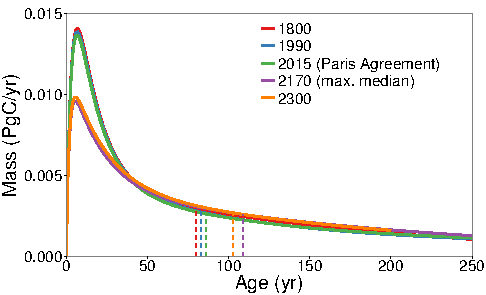
\includegraphics[width=\linewidth]{images/content/ftt.pdf}
	  \end{center}
	\end{column}
	\setlength{\rc}{\the\dimexpr (\textwidth-\lc) \relax }
	\begin{column}{\rc}
    \begin{minipage}{0.95\rc}
    Forward transit-time densities of $1\, \text{PgC}$ %$1\, \si{\peta\gram\carbon}$ 
      hypothetically injected into the atmosphere in the years 1800 (red), 1990 (blue), 2015 (green), 2170 (purple), and 2300 (orange).
      The orange curve ends at the age of 200, because our simulation only lasts until the year 2500.
      The medians (dashed vertical lines) increase until the year 2170 and then start decreasing.
      \label{fig:ftt}
    \end{minipage}
	\end{column}
\end{columns}
